\chapter{Temporal ANN and Knowledge Tracing}\label{ch:kt_background}
In this chapter, we present the relevant background for Part II, the incorporation of IRT into knowledge tracing. The application of knowledge tracing extends educational measurement to a more dynamic setting. Rather than receiving all student's responses to an assessment after the exam is completed, data is gathered in real-time as the student progresses through each question. So the data is structured as a time series, and the task is to track student knowledge as more information comes in.

Because of the different format of data, this chapter first reviews popular neural networks which are equipped to deal with time series data. Though these ANN are often referred to as ``recurrent'' neural networks, we avoid that terminology because not all of them have a truly recurrent structure (see Section \ref{sec:transformers}). Instead, the we classify these neural networks as ``temporal neural networks,'' (TNN) since they relate to time-dependent data.

After providing background on various TNN in a more general setting, a literature review of previous knowledge tracing methods is provided. Specifically, we explain how TNN are adapted to better fit the knowledge tracing application, including the methods for representing student interaction data and modifications to TNN architecture.

\section*{Temporal Neural Networks}
In many deep learning applications such as video processing, natural language processing, or dynamical systems, the observed data is time-dependent \cite{kahou2015, gilpin2020, vaswani2017}. In such datasets, a single observation of $n$ features can not represented as a vector $\vect x_0 \in \R^n$, but must take into account the $T$ different measurements of the $n$ features, each taken at a different timestep $1 \leq t \leq T$. As such, a data point is represented as a matrix $X_0 \in \R^{n \times T}$, where the $t$-th column of $X_0$ gives a snapshot of the observation at time $t$. For example, in the natural language application, a data point $X_0$ may represent a sentence or paragraph, and a column $\vect x_{0,t}$ of $X_0$ would represent a word in that sentence/paragraph.

\section{Recurrent Neural Networks}
Recurrent Neural Networks (RNN) are the most simple adaptation of neural networks to deal with time-series data. Recall that a regular feed-forward neural network layer of size $h$ takes an input vector $\vect x \in \R^n$ and outputs
\begin{equation}
  \vect y = f( W\vect x + \vect b)
  \label{eq:ffn_layer}
\end{equation}
where $W \in \R^{h \times n}$ and $\vect b \in \R^h$ are trainable parameters, and $f$ is a non-decreasing activation function \cite{sharma2020}. 

In the time-dependent setting, let $\vect x_t$ be a column of an input $X$. A basic recurrent layer calculates 
\begin{equation}
  \begin{split}
    \vect h_t &= \tanh(W_{hh}\vect h_{t-1} + W_{hx}\vect x_t + \vect b_h) \\
    \vect y_t &= \sigma(W_{hy}[\vect x_t, \vect h_t] + \vect b_y)
\end{split}
  \label{eq:rnn_layer}
\end{equation}
where $W_{hh} \in \R^{h\times h}$, $W_{hx}\in \R^{h\times n}$, $\vect b_h \in \R^h$, $W_{hy} \in \R^{h \times (h+n)}$, and $\vect b_y \in \R^h$ are trainable parameters \cite{elman1990}. The notation $[\vect x_t, \vect h_t]$ refers to vector concatenation, and $\tanh(\cdot)$ and $\sigma(\cdot)$ refer to the hyperbolic tangent and sigmoid activation functions, respectively, detailed further in Appendix \ref{apdx:activation_fcns}. Note that this allows the output $\vect y_t$ to include information from previous timesteps. A visualization of an unfolded RNN is shown in Figure \ref{fig:rnn_visual}.

\begin{figure}[h]
  \centering
  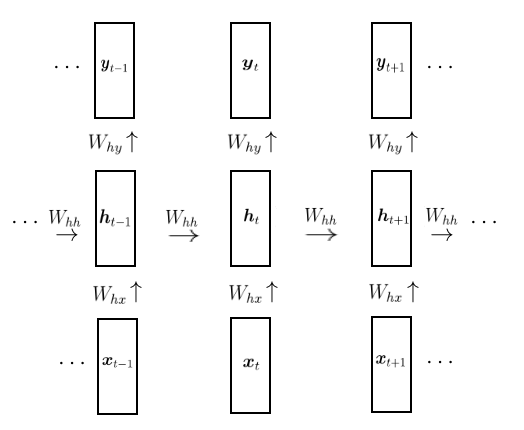
\includegraphics[width=.5\textwidth]{img/rnn_visual.png}
  \caption{Architecture of a recurrent neural network. Note that the same weights matrices $W_{hx}$, $W_{hh}$, and $W_{hy}$ are used in each timestep.}
  \label{fig:rnn_visual}
\end{figure}

One issue that RNN face is the exploding or vanishing gradient problem \cite{bengio1994}, where the norm of the gradient can become very large or very small during training. This is due to the fact that partial derivatives calculated during back-propagation between hidden states at time $t_1$ and $t_2$ is found by a product of $(t_2 - t_1)$ Jacobian matrices \cite{pascanu2013}. As the difference between $t_1$ and $t_2$ increases, the corresponding partial derivatives $\displaystyle\frac{\partial \vect h_{t_1}}{\partial \vect h_{t_2}}$ can exponentially grow or exponentially decay in norm.

Related to the exploding/vanishing gradient issue, RNN experience difficulty in retaining important information for multiple timesteps is difficult. For example, if an important phenomena happens to data point $X_0$ at time $t$, then that information should still influence the values of $\vect h_{t+10}$ and $\vect y_{t+10}$. But the structure described in Equation \ref{eq:rnn_layer} and Figure \ref{fig:rnn_visual} causes the impact of $\vect x_t$ and $\vect h_t$ to fade over time.


\section{Long Short-Term Memory Networks}\label{sec:lstm}
To combat the problems of RNN, Long Short-Term Memory (LSTM) networks were developed by Hochreiter and Schmidhuber \cite{hochreiter1997}. This architecture introduces element-wise multiplication and addition operations along with multiple trainable weights matrices which allows for tracking long-term dependencies. An LSTM layer computes a ``cell state'' vector $\vect c_t$, in addition to the hidden layer representation $\vect h_t$. This cell state is updated at each timestep to ``remember'' important information and ``forget'' frivolous information.

The LSTM structure also addresses the exploding/vanishing gradient of RNN. The presence of the cell state $\vect c_t$ ensures that calculating derivatives of long-range dependencies do not include many matrix multiplications \cite{hochreiter1997}.

A single cell of an LSTM can be compared to the middle block in Figure \ref{fig:rnn_visual} containing $\vect h_t$ of an RNN. At time $t$ and given an input $\vect x_t$, previous hidden state $\vect h_{t-1}$, and previous cell state $c_{t-1}$, an LSTM cell uses four trainable weights matrices and four element-wise operations. First compute the ``forget'' vector $\vect f_t$, the ``update'' vector $\vect u_t$, the ``add'' vector $\vect a_t$, and the ``filter'' vector $\vect g_t$.
\begin{equation}
\begin{split}
  \vect f_t &= \sigma(W_f [\vect x_t, \vect h_{t-1}] + \vect b_f) \\
  \vect u_t &= \sigma(W_u [\vect x_t, \vect h_{t-1}] + \vect b_u) \\
  \vect a_t &= \tanh(W_a [\vect x_t, \vect h_{t-1}] + \vect b_a) \\
  \vect g_t &= \sigma(W_g [\vect x_t, \vect h_{t-1}] + \vect b_g)
\end{split}
  \label{eq:lstm_vects}
\end{equation}

The first three vectors in Equation \ref{eq:lstm_vects} are used to perform element-wise operations on $\vect c_{t-1}$ to produce the next cell state $\vect c_t$, and $\vect g_t$ is used in updating $\vect h_t$. Notice that the sigmoid activation function $\sigma(\cdot)$ maps small inputs to near $0$ and large inputs to near $1$, while the hyperbolic tangent activation function $\tanh(\cdot)$ maps small inputs to near $-1$ and large inputs to near $1$. 

Using $\vect f_t$, unimportant aspects (elements in $\vect f_t$ near zero) of $\vect c_{t-1}$ are forgotten:
\begin{equation}
  \tilde{\vect c}_{t-1} = \vect c_{t-1} \times \vect f_t
  \label{eq:lstm_forget}
\end{equation}
where $\times$ is element-wise multiplication. Next, $\vect u_t$ decides what information to update (elements in $\vect u_t$ near one), and $\vect a_t$ gives the value (an increase or decrease) of the information to be updated:
\begin{equation}
  \vect c_t = \tilde{\vect c}_{t-1} + \left( \vect u_t \times \vect a_t \right)
  \label{eq:lstm_update}
\end{equation}
where $+$ and $\times$ are element-wise addition and multiplication, respectively. Lastly, compute the next hidden state using $\vect g_t$, which filters the information to be passed to the next network layer and next timestep:
\begin{equation}
  \vect h_t = \tanh(\vect c_t) \times \vect g_t
  \label{eq:lstm_filter}
\end{equation}

\begin{figure}[h]
  \centering
  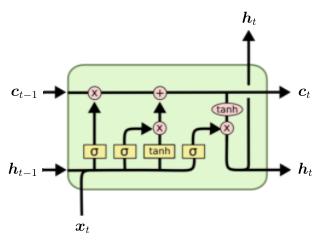
\includegraphics[width=.5\textwidth]{img/lstm_visual}
  \caption{Architecture of a single LSTM cell \cite{olah2015}. Trainable matrix multiplication followed by an activation function are in yellow boxes, and element-wise operations without learned parameters are in red ovals.}
  \label{fig:lstm_visual}
\end{figure}

The architecture of a single LSTM cell is visualized in Figure \ref{fig:lstm_visual}. The forget vector acts as a gate which allows/disallows past information to persist over time, while the update and add vector grabs the data from the current input which is worth updating and remembering.


\section{Transformers and Attention}\label{sec:transformers}
Though LSTM networks presented a significant breakthrough in natural language processing (NLP), they have been quickly surpassed in the application of language modeling by attention-based methods. These models forgo the recurrent structure of information flow seen in RNN and LSTM for feed-forward layers and similarity scores between time steps. For example, calculating a similarity score between each pair of words in a sentence can help extract deeper context in language models such as transformers \cite{vaswani2017}.

While transformers are large neural networks with many components and parameters, they lean heavily on a simple attention mechanism. Given an $n$-dimensional feature vector $\vect x_t$ at each timestep $1\leq t\leq T$, define three trainable matrices $W_q, W_k, W_v \in \R^{n\times d}$. These are used to obtain a \textit{query}, \textit{key}, and \textit{value} vectors $\vect q_t$, $\vect k_t$, and $\vect v_t$ for each timestep. 

The query and key vectors are representations of the observations $\vect x_t$ which are used to quantify the relationship between observations $\vect x_{t_1}$ and $\vect x_{t_2}$, with the distinction between them being that a query typically refers to the current timestep. In other words, if event $t$ just occurred, we may be interested in comparing $\vect q_t$ to a previous observation $\vect k_{t-1}$. The value vector $\vect v_t$ is a representation of $\vect x_t$ which holds deeper, more contextual information of the observation. Note that $\vect q_t$, $\vect k_t$, and $\vect v_t$ can be stacked into matrices $Q,K,V \in \R^{T\times d}$. 

The queries and keys are used first, to calculate the correlation between observation $t$ and all other timesteps:
\begin{equation}
  \vect c_t = \text{softmax}\left(\frac{K \vect q_t}{\sqrt{d}} \right) \in \R^T
  \label{eq:attn_cor}
\end{equation}
Notice that the matrix multiplication $K \vect q_t$ in Equation \ref{eq:attn_cor} is simply $T$ individual dot-product computations. So the $i$-th entry of $\vect c_t$ gives the similarity between the input at time $t$ and the input at time $i$. The softmax function $\text{softmax}(z_i) = \displaystyle\frac{e^{z_i}}{\sum_{j=1}^T e^{z_j}}$ rescales the dot product calculations so that the sum of the entries of $\vect c_t$ is equal to 1. 

In applications where an input $\vect x_{t_1}$ is not allowed to see information of future inputs $\vect x_{t_2}$, $t_1<t_2$, the corresponding entries of $K\vect q_{t_1}$ are masked to be $-\infty$. This causes the entries $c_{ti} = 0$ when $i > t$. It is also worth pointing out that this correlation score is not symmetric -- the dot product between two queries and keys of the timesteps $\vect x_t$ and $\vect x_{t'}$ is not equal: $\vect k_{t'}^\top \vect q_t \not = \vect k_t^\top \vect q_{t'}$. To understand why this is desirable, consider the NLP application and the sentence ``The dog is happy.'' Correlation between a query for ``The'' and a key for ``dog'' should be different from the reverse. When querying ``The,'' we wish to know what ``The'' is referring to (the dog). But when querying ``dog,'' we wish to know something about the dog (it is happy) -- the article ``The'' is unimportant in this sense.

Next, the attention is calculated as 
\begin{equation}
  \vect a_t = V \vect c_t \in \R^d
  \label{eq:attn}
\end{equation}
The attention vector $\vect a_t$ is a weighted sum of the value vectors of each other timestep, weighted by the correlation scores in Equation \ref{eq:attn_cor}. The attention calculation can also be written more generally for all timesteps at once:
\begin{equation}
  A = \text{softmax}\left(\frac{QK^\top}{\sqrt{d}} \right) V \in \R^{T \times d}
  \label{eq:attn_matrix}
\end{equation}

In attention networks, the attention vectors $\vect a_t$ are individually sent through feed-forward layers. For example, transformers calculate attention and then use three feed-forward layers in a single ``block'' \cite{vaswani2017}. These blocks are stacked on top of each other up to six times to obtain deeper and deeper contextualization of the input sequence \cite{dai2019}. Eventually, this contextualization is plugged into a final prediction layer, depending on the application.

It should be pointed out that transformers and attention networks were developed specifically for the NLP application. So in this case, a sequence of $T$ inputs represents a sentence of length $\leq T$ and an input vector $\vect x_t$ is an $n$-dimensional learned representation of a single word \cite{mikolov2013}. Then the correlation score in Equation \ref{eq:attn_cor} is quantifying the relationship between pairs of words in the sentence.


\section*{Knowledge Tracing Overview}
Knowledge Tracing (KT) is a task introduced by Corbett and Anderson in 1995 \cite{corbett1995}. Their goal was to model the changing knowledge state of students as they progress through an online intelligent tutoring program. This tutoring system helps students practice writing computer programs by testing them on various rules, such as correct use of in-built functions, and providing feedback on their mistakes. The model tracks each student's knowledge as being in either a learned or unlearned state for each rule. After each interaction, there is a probability $P(T)$ that a student makes the transition from the unlearned state to the learned state.

The probability that a student has learned a particular rule at timestep $t$ is given by
\begin{equation}
  P(L_t) = P(L_{t-1} | \text{evidence}) + (1 - P(L_{t-1} | \text{evidence})) \cdot P(T),
\label{eq:kt}
\end{equation}
where ``evidence'' refers to whether or not previous interactions were correct or not \cite{corbett1995}. The probability of student performing the $t$-th task correctly is 
\begin{equation}
  P(c_t = 1) = P(L_t) \cdot (1 - P(s)) + (1 - P(L_t))\cdot P(g)
  \label{eq:kt_prob_correct}
\end{equation}
where $P(s)$ is the probability that the student slips (makes a silly mistake) and $P(g)$ is the probability that the student randomly guesses correctly. The parameters $P(T)$, $P(g)$, and $P(s)$ are estimated using hidden Markov model, along with an initial value $P(L_0)$. Then Equation \ref{eq:kt} is updated via Bayes' rule.

In recent years, Bayesian Knowledge Tracing (BKT) has been overcome by deep learning methods. The popularity of deep neural networks has brought black-box models that yield high accuracy. Many of these methods, detailed in Section \ref{sec:kt_lit}, do not provide a concrete measure of student ability over time. Instead, the only way to track student knowledge is through the predicted probability of them answering questions correctly at a given timestep. 

In Chapter \ref{ch:kt_methods}, new methods using neural networks are presented which produce comparable predictive power to deep learning methods, while providing explainable models with links to Item Response Theory.


\section{Knowledge Tracing Literature Review}\label{sec:kt_lit}
In the modern knowledge tracing application, data is provided as a sequence of student interactions $x_t = (q_t, c_t)$, $0 \leq t \leq L$. $L$ is a hyperparameter denoting the maximum length of the sequence -- since the number of interactions for each student is different, response sequences shorter than $L$ are padded with null interactions, and response sequences of length longer than $L$ are wrapped into multiple sequences. For example, if $L=128$ and a particular student answers $161$ questions, then this student's interactions will be split into two separate sequences of length $81$ and $80$.

The tag $q_t$ indexes a particular question (item) in the available question bank, and $c_t \in\{0,1\}$ indicates whether the question was answered incorrectly or correctly. So for a learning system with $n$ available questions, there are $2n$ distinct interactions for the tuple $x_t$. The knowledge tracing task is to predict $c_{t+1}$ given all previous interactions. Mathematically, the quantity of interest is the probability 
\begin{equation}
  P(c_{t+1} = 1 | (q_0,c_0), (q_1,c_1),\ldots,(q_t, c_t), (q_{t+1}, ?)).
  \label{eq:kt_prob}
\end{equation}
Most neural networks optimize the predicted probability in Equation \ref{eq:kt_prob} by  minimizing the cross-entropy loss function, as described in Equation \ref{eq:cross_entropy}.

\subsection{Deep Knowledge Tracing}
In 2015, the first use of neural networks for knowledge tracing was introduced by Piech et al. \cite{piech2015}. Deep Knowledge Tracing (DKT) utilizes recurrent neural networks (RNN) and Long-Short Term Memory (LSTM) neural networks to predict a student's success on future questions, given a sequence of previous interactions. 

Similar to natural language processing, tokens (student interactions) need to be represented as a $d$-dimensional vector. DKT does this by one-hot encoding the interactions in the input layer to have shape $(2n+1, L)$,  and linearly mapping to a hidden layer of shape $(d, L)$. Each interaction in the sequence is treated independently in this layer. The input layer shape is $2n+1$ for each of the possible $2n$ interactions, along with space for an additional padding token representing a null interaction (for response sequences of length $< L$.

The architecture of DKT is as follows: The one-hot encoding input layer is followed by a $d$-dimensional embedding. Then, an LSTM layer of size $d$, and a feed-forward output layer with $n$ nodes. The final layer uses a sigmoid activation function, and the output at each node represents the probability of answering the corresponding item correctly at the given timestep. To calculate loss, only the item tag for the next interaction and corresponding output node is used in the cross-entropy loss calculation. Output nodes corresponding with items that don't match the interaction sequence are masked out.

  \subsection{Dynamic Key-Value Memory Networks}\label{sec:dkvmn}
A more sophisticated neural network approach to knowledge tracing was introduced by Zhang et al. with Dynamic Key-Value Memory Networks (DKVMN) \cite{zhang2017}. They modify a memory-augmented neural network (MANN) in order to fit into the knowledge tracing framework. A MANN is a temporal neural network which uses a value matrix $M^v$ stored in memory for each student. The entries in $M^v$ are updated in each timestep with element-wise addition and multiplication, similar to an LSTM in Section \ref{sec:lstm}. The output is a probability dependent on the previous value of $M^v$ in timestep $t-1$, as well as the current neural network input in timestep $t$.

In DKVMN, there is some added interpretability by requiring the number of columns of $M^v$ to be equal to the number of knowledge concepts $K$. In this way, the columns of $M^v$ offer an $h$-dimensional representation of the student's skill. DKVMN splits the computations into two parts: \textit{read} from $M^v$ to make a prediction of answering an item correctly, and \textit{write} to $M^v$ to update its information after observing a true outcome. The predictive part inputs only an exercise tag $q_t$ without the true response $c_t$. The question tag is linearly embedded into a vector $\vect k_t$, so that $\vect k_t$ is a representation of question $q_t$, and is then multiplied by a learned matrix $M^k$ and softmaxed: 
\begin{equation}
  \vect w_t = \text{softmax}\left( M^k \vect k_t \right)
  \label{eq:dkvmn_weight}
\end{equation}

This creates a vector $\vect w_t$, where entry $i$ in $\vect w_t$ represents the correlation weight between the question $q_t$ and memory slot $i$. This process of taking the dot product between an item embedding and a trainable matrix then softmaxing is similar to the concept of attention (described in Section \ref{sec:transformers}), used in popular NLP techniques such as transformers \cite{vaswani2017}.

Next, \textit{read} from the value matrix by computing 
\begin{equation}
  \vect r_t = \sum_{i=1}^K \vect w_t(i) M_t^v(i).
  \label{eq:dkvmn_read}
\end{equation}
Note that $\vect r_t$ is simply a weighted sum of the columns of $M^v$ and can be treated as a summary of the student's predicted mastery level of exercise $q_t$. Next, the item embedding $\vect k_t$ is appended to the read content $\vect r_t$ and fed forward through two linear layers. The first uses a $\tanh$ activation function, and the output $p_t$ produces a single node with sigmoidal activation. In this way, the single value $p_t$ represents the probability that the student will answer item $q_t$ correctly at timestep $t$.

The second part of DKVMN is to \textit{write} new values into $M^v$ based on the true response of students. Different from the prediction phase, the full tuple $(q_t,c_t)$ is embedded into a vector $\vect v_t$. The manner in which $M^v$ is updated is actually similar to that of an LSTM, allowing for ``remembering'' and ``forgetting''. $\vect v_t$ is multiplied by two trainable matrices to produce an ``erase'' vector $\vect e_t$ and an ``add vector'' $\vect a_t$. The erase vector has a sigmoidal activation function, so that values near zero do not get erased much at all, and values near one are mostly erased. The add vector uses a $\tanh$ activation function, so memory slots in $M^v$ can either be increased or decreased. Finally, the columns of the memory matrix are updated via
\begin{equation}
  M_{t}^v(i) = (M_{t-1}^v(i) [\vect 1 - \vect w_t(i) \vect e_t] ) + \vect w_t(i) \vect a_t
  \label{eq:update_dkvmn}
\end{equation}
Note that the correlation weights $\vect w_t$ computed in the predictive step are again used to determine \textit{how much} of memory slot $i$ should be updated.

DKVMN's use of a matrix stored in memory allows for longer range dependencies than RNN or LSTM. There is also a bit of interpretability in this method, since a single column of the memory matrix $M_t^v$ gives an $h$-dimensional representation of a single skill for the student at time $t$. However, it cannot be determined \textit{which} skill the column represents, as they could be permuted in any order. Additionally, if a student answers each available item, then stacking each weights vector $\vect w_t$ into a matrix $W = \{\vect w_t\}_{t=1}^L$ should result in a matrix similar to the item-skill association $Q$-matrix. But again, the columns of this ``learned $Q$-matrix'' $W$ are in no particular order, and can be difficult to interpret.

\subsubsection{Deep-IRT}
Deep-IRT, proposed by Chun-Kit Yeung \cite{yeung_2019}, modifies the DKVMN architecture to allow a connection with Item Response Theory. Specifically, two separate feed forward layers are inserted representing $\theta_{tk}$, a student's $k$-th ability at time $t$ and concept difficulty $\beta_k$. Then the output probability is not another linear layer (as in DKVMN), but is instead a function of $\theta_{tk}$ and $\beta_k$:

\begin{equation}
  p_t = \frac{1}{1 + \exp\left( \beta_k - 3\cdot \theta_{tk} \right)}
  \label{eq:deep_irt_prob}
\end{equation}

These modifications provide a link to the Rasch model in Equation \ref{eq:rasch}. The multiplication by 3 is for practical reasons to re-scale $\theta_{tk}$. However, note that in Equation \ref{eq:deep_irt_prob}, the difficulty parameter is on the \textit{concept} level, and not the \textit{item} level like the Rasch model (and other IRT models). Though Deep-IRT doesn't seek to directly approximate the Rasch model, the modifications to DKVMN still adds significant interpretability to the deep neural network.


\subsection{Self-Attentive Knowledge Tracing}\label{sec:sakt}
In the field of natural language processing (NLP), the most state-of-the-art methods utilize the self-attention mechanism \cite{vaswani2017}, which relies on calculating the correlation between pairs of words in a sentence. Popular models such as BERT \cite{bert} and GPT-3 \cite{gpt3} are both transformer-based neural networks for NLP which heavily depend on attention. Self-Attentive Knowledge Tracing (SAKT) adapts this concept for the knowledge tracing task \cite{pandey2019}. 

Similar to other deep learning methods, at timestep $t$, SAKT first embeds each interaction $(q_i, c_i)$, $i<t$ into a learned $d$-dimensional vector $\vect m_i$. Additionally, like DKVMN, the current question $q_t$ without the response is also embedded into a $d$-dimensional vector $\vect e_t$. 

The exercise embedding $\vect e_t$ is multiplied by a weights matrix to obtain a \textit{query} vector $\vect q_t = W_{q} \vect e_t$. The interaction embedding $\vect m_i$ is used to create two vectors: a \textit{key} vector $\vect k_i = W_{k} \vect m_i$ and a \textit{value} vector $\vect v_i = W_v \vect m_i$. 

The general idea is that $\vect k_i$ serves as the identifier of a past interaction, and $\vect q_t$ serves as an identifier for the current exercise. If the two exercises are similar in content, then the dot product between these two vectors should be large. The value vector $\vect v_i$ holds more abstract information about the corresponding interaction. The keys and values are organized into matrices $K$ and $V$. We calculate the attention
\begin{equation}
  \vect a_{t} = \text{softmax}\left(\frac{K \vect q_t}{\sqrt{d}} \right) V
  \label{eq:attn_sakt}
\end{equation}

The value $\frac{K \vect q_t}{\sqrt{d}}$ yields a vector where the $i$-th entry is the dot product between the current exercise query $\vect q_t$ and an interaction key $\vect k_i$. This is scaled by dimension and softmaxed, resulting in a weighted sum of the value vectors $\vect v_i$.

The attention value $\vect a_t$ is sent through a few feed-forward layers, resulting in a vector $\vect f_t = \text{FFN}(\vect a_t)$. The output layer is $p_t = \sigma(\vect f_t W + \vect b)$, the probability that the student will answer the current exercise $q_t$ correctly, where $W$ and $b$ are trainable parameters.


\subsection{Performance Factors Analysis}
An earlier approach to knowledge tracing was proposed by Pavlik et al. in 2009 with Performance Factors Analysis (PFA) \cite{pavlik2009}. The general idea is that a student's learning at a given timestep is a function of the student's past interactions with items related to various knowledge concepts. Specifically, the logit of student $j$ answering item $i$ correctly is a linear combination of concept difficulty, previous successes, and previous failures:
\begin{equation}
  \begin{split}
    \log \frac{p}{1-p} &= \sum_{k \in K_i}(\beta_k + \gamma_k s_{jk} + \rho_k f_{jk}) \\
  p(c_i = 1 | k\in \text{K}_i, \vect s_j, \vect f_j) &= \sigma\left(\sum_{k \in K_i}(\beta_k + \gamma_k s_{jk} + \rho_k f_{jk}\right)
  \end{split}
  \label{eq:pfa}
\end{equation}

In Equation \ref{eq:pfa}, $\text{K}_i$ is a set indicating which knowledge concepts are required for item $i$, the trainable parameter $\beta_k$ represents concept $k$'s difficulty, and $\gamma_k$ and $\rho_k$ serve as trainable weights. $s_{jk}$ and $f_{jk}$ track the prior successes and failures, respectively, of student $j$ on concept $k$. At timestep $t$, we can write $s_{jk}$ and $f_{jk}$ as 
\begin{equation}
  \begin{split}
    s_{jk} = \sum_{i<t} \chi_{(c_i=1)} \cdot \chi_{(k \in \text{K}_i)} \\
    f_{jk} = \sum_{i<t} \chi_{(c_i=0)} \cdot \chi_{(k \in \text{K}_i)}
  \end{split}
  \label{eq:pfa_indicator}
\end{equation}
where $\chi$ is the indicator function. For example, $\chi_{(k\in \text{K}_i)}$ indicates whether the previous item $q_i$, $i<t$, required knowledge concept $k$ or not.

The parameters $\beta_k$, $\gamma_k$, and $\rho_k$ are learned so that they maximize the log-likelihood of the given dataset. This is a well-studied problem, as the form of Equation \ref{eq:pfa} is essentially a logistic regression. Note that similar to Deep-IRT, PFA focuses on the concept-level, rather than item-level, parameters. 

\subsection{Deep Performance Factors Analysis}
Recent work has related PFA to the self-attention mechanism used in SAKT described in Section \ref{sec:sakt}. Pu et al. \cite{deep_pfa} developed Deep Performance Factors Analysis (DPFA) and a new characterization of the weight parameters $\gamma_k$ and $\rho_k$, using learned item embeddings $\vect e_i$ for each question $q_i$.

For the current question $q_{t+1}$, the attention between previous exercises is $A_{i,t+1} = \vect e_i^\top \vect e_{t+1}$, for $i \leq t$. Note that this incorporates ideas from SAKT, but the attention is symmetric. More recent interactions are taken into account by calculating $d_{i,t+1} = -a(t-i+1)+b$, where $a$ and $b$ are trainable parameters. Then the relevance of a past item depends on the dot product similarity and how long ago the interaction took place:
\begin{equation}
  w_{t+1} = \text{softmax}(A_{:,t+1} + d_{:,t+1})
  \label{eq:time_bias_attn}
\end{equation}

The mastery of knowledge concepts after a student completes interaction $(q_i, c_i)$ is given as $\vect v_i = [v_i^0, v_i^1] \in \R^2$. The numbers $v_i^0$ and $v_i^1$ represent the expected mastery of the skills for item $i$ if the item is answered incorrectly or correctly, respectively. DPFA gives the probability of a student answering item $q_{t+1}$ correctly as
\begin{equation}
  p_{t+1} = \sigma\left( \beta_{t+1} + \sum_{i \leq t} \left( \chi_{(c_i=0)}\cdot w_i v_i^0 + \chi_{(c_i=1)} \cdot w_i v_i^1 \right) \right)
  \label{eq:dpfa}
\end{equation}
where $\beta_{t+1}$ corresponds to the difficulty of the current item and $\sigma(\cdot)$ is the sigmoid function. In comparison with regular PFA in Equation \ref{eq:pfa}, DPFA substitutes the terms $\chi_{(c_i=0)}\cdot w_i v_i^0$ for $\rho_k f_k$ and substitutes $\chi_{(c_i=1)} \cdot w_i v_i^1$ for $\gamma_k s_k$.

